Given a sentence $\mathcal{S}$ as a $n$-length sequence of tokens, $\mathcal{S} = \langle w_1, w_2 \ldots w_n \rangle$, the goal of this module is to output a list of spans (mention tuples) $\langle s, e\rangle$ where $s$ and $e \in [1, n]$ are the \textit{start} and \textit{end} index respectively. 
Note that the mention tuples are not associated with an entity type. 

We formulate this as a QA task and train a model to extract all required mention spans from a given sentence. Since the goal is to detect the spans irrespective of their entity type, we use a generic query statement ``\textit{Extract important entity spans from the following text}'' prefixed with the input sentence. Our query also indicates that we are not interested in all entity spans, only the ones we train the model to deem important. The model outputs \texttt{B}, \texttt{I}, \texttt{O} or \texttt{E} labels for each token representing the span using \texttt{BIOE} tagging scheme. The bottom diagram in Figure \ref{fig:framework} shows an example sentence processed by this module.

\spandetect{} must ensure that it identifies mention spans with accurate boundaries. This is because \spanclass{} just assigns an entity type to the span and does not adjust its boundaries. In fact, inaccurate mention boundaries could lead to sub-optimal predictions. For example, \textit{Apple} is a \type{Fruit}, while \textit{Apple Inc} is an \type{Org}.

Many domain-specific terms occur rarely and may not have a good semantic representation in the underlying BERT model. However, they may have  shared patterns at character-level (for example, chemical formulas). \cite{boukkouri2020characterbert} propose a character-level CNN layer instead of the WordPiece tokenizer at the input stage to the BERT model to better capture such terms. Motivated by this design, we explicitly model character sequences and intrinsic patterns within terms as additional features along with the BERT output.
 
\subsubsection{Character Modeling} Each token output from WordPiece Tokenizer is simultaneously fed to five one-dimensional CNNs with kernel sizes of $1$ to $5$, each having $16$ filters and $50$ input channels. The CNNs are designed to perform depthwise convolution over the characters of the token, each character being represented by a $50$ dimensional embedding. Character-level outputs from the CNN are max-pooled to get a token-level representation. Outputs from multiple CNNs are concatenated and passed through a linear layer with ReLU activation to get an overall $768$-dimensional feature vector.
    
\subsubsection{Pattern Modeling} Each token from WordPiece Tokenizer is converted to a pattern encoding to group together rare tokens which share similarities. The patterns are fed to a character CNN setup (similar to the one above) and then to a bidirectional LSTM with $256$ hidden dimensions to output a $512$-dimensional contextual pattern feature vector for each token.

The pattern encoding is created by mapping all uppercase tokens to a single character, \texttt{U}, all lowercase tokens to \texttt{L}, all digit tokens to \texttt{D}. BERT's special tokens, ``[CLS]'' and ``[SEP]'' are mapped to \texttt{C} and \texttt{S} respectively. If a token contains a combination of uppercase, lowercase, digit and/or special characters then we map its lowercase characters to \texttt{l}, uppercase ones to \texttt{u} and digits to \texttt{d}. This way, we maintain the intrinsic pattern and length information of the token. For example, this encoding scheme converts ``NER'' and ``BERT'' both to \texttt{U}, ``2Q-NER'' to \texttt{du-uuu} and ``CaSO4'' and ``MgSO4'' are both mapped to \texttt{uluud}.

Finally, the character and pattern features are concatenated with the BERT output for the token and fed to a final classifier linear layer
as shown in  Figure~\ref{fig:span_detection}.
%Hereafter, we denote the character and pattern features as \method{CharPattern}.
    
% This character and pattern modeling is a customization over the vanilla BERT model, adapted to learn better mention boundaries. \comment{maybe? we could say this customization is more effective when done on span detection rather than full NER BERT? :} Note that we could do this because we split our task up into simpler sub-tasks and decided to tackle them one at a time. \comment{can give table in appendix to show some example boundary detection issues motivating char-pattern modeling}

\begin{figure}[h!]
    \centering
    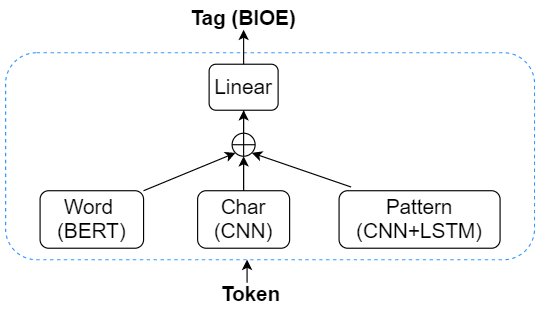
\includegraphics[width=0.9\linewidth]{span_det7.png}
    \caption{Token-level schematic architecture of \spandetect{}}
    \label{fig:span_detection}
\end{figure}
